\graphicspath{{content/3_results/figures}}
\section{Motor Controller}

\subsection{Simulation}

The results of the simulation for the two motor controller stages can be found below.

\begin{figure}[!htb]
  \centering
  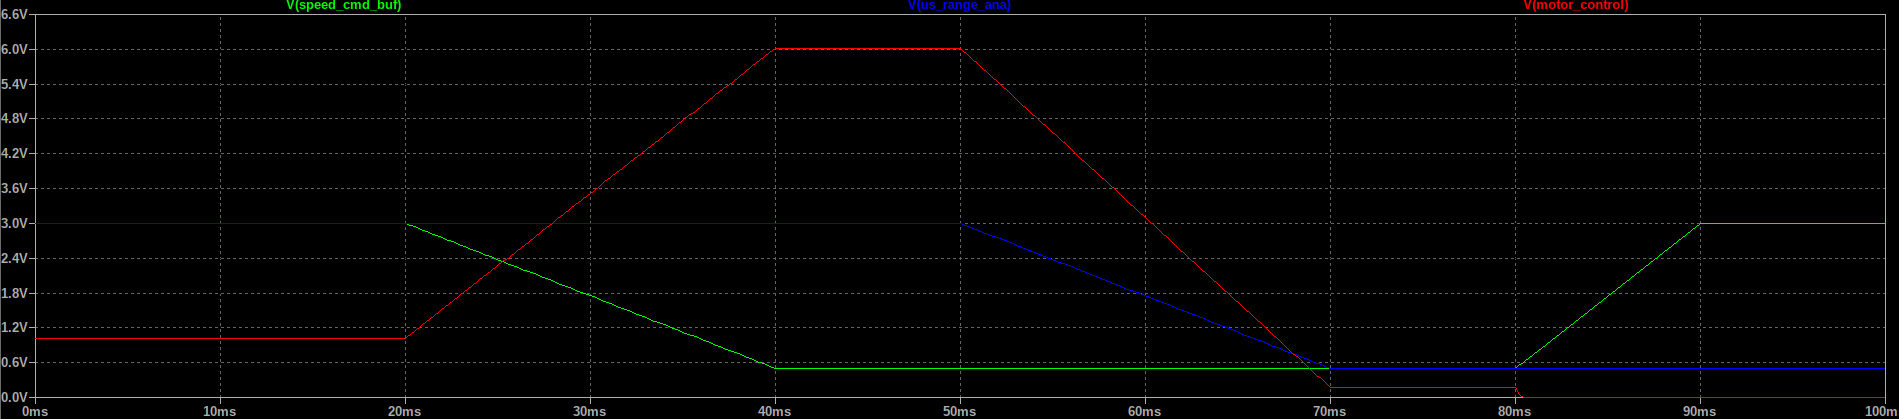
\includegraphics[width=0.8\textwidth]{motorController_sim_subtractor_output}
  \caption{Motor Controller Output of Subtractor Stage}
  \label{fig:motorController_sim_subtractor_output}
\end{figure}

\begin{figure}[!htb]
  \centering
  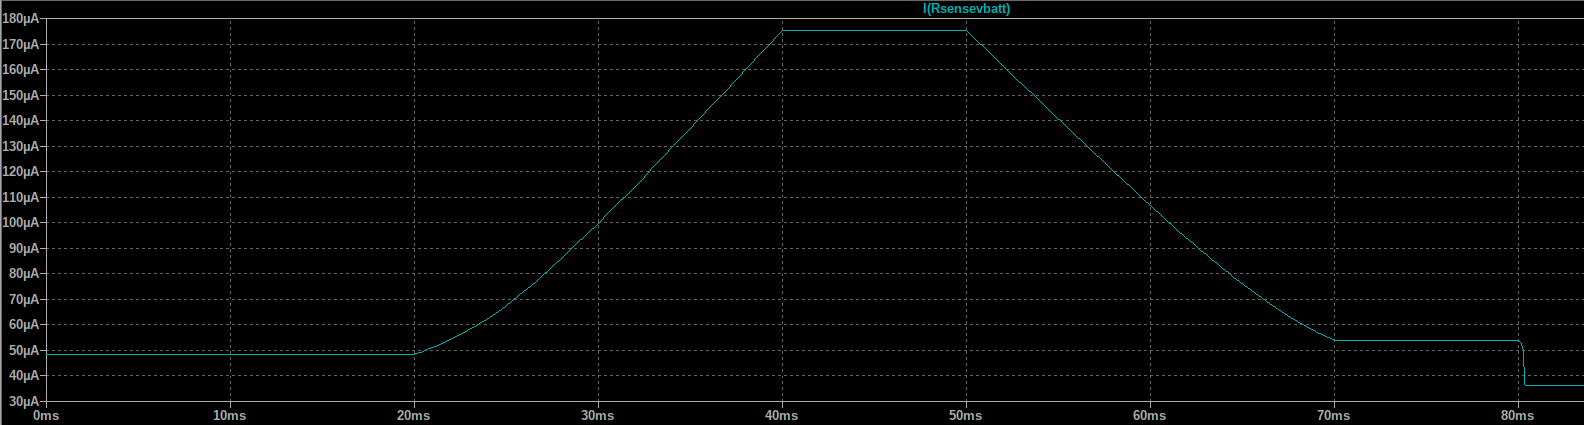
\includegraphics[width=0.6\textwidth]{motorController_sim_subtractor_currentDraw}
  \caption{Motor Controller Current Draw of Subtractor Stage}
  \label{fig:motorController_sim_subtractor_currentDraw}
\end{figure}

\begin{figure}[!htb]
    \centering
    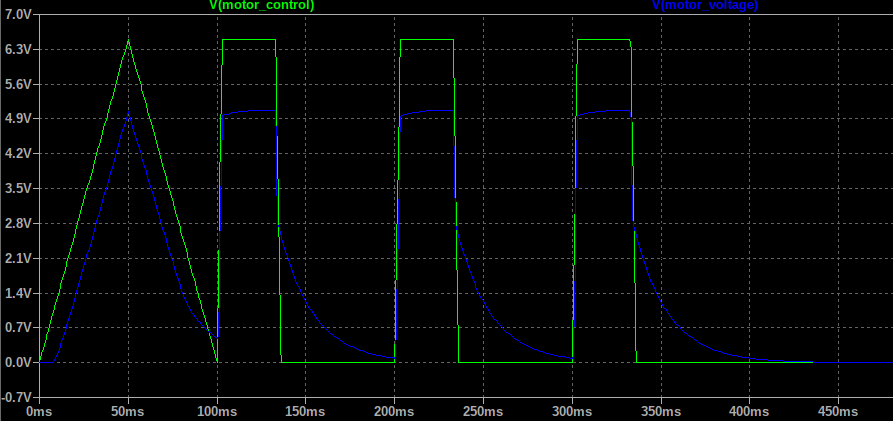
\includegraphics[width=0.45\textwidth]{motorController_sim_power_output}
    \caption{Motor Controller Output of Power Stage}
    \label{fig:motorController_sim_power_output}
  \end{figure}

As can be seen, specifications were complied to:
\begin{itemize}
    \item A "low speed" command (3 V) and "no object" command (3 V) results in a low controller command ($< \SI{1.8}{V}$).
    \item A "high speed" command (0.5 V) and "no object" command (3 V) results in a high controller command. The output, however, only reaches 6 V
          due to a different input range. A simulation with $V_{speed} = \SI{0.1}{V}$ and $V_{range} = \SI{3.3}{V}$ shows that the output saturates at 7.2 V.
    \item The current draw of the subtractor is as designed i.e. $< \SI{400}{\micro\ampere}$, and therefore the total current is $< \SI{1.5}{A}$ due to the
          maximum motor current draw of $\SI{1}{A}$.
    \item The drop from the motor control command to the motor is $\SI{1.4}{V}$, meaning the designed minimum of $\SI{1.8}{V}$ will ensure the motor
          has $V_{motor} < \SI{0.5}{V}$.
\end{itemize}

\subsection{Measured}

Voltage measurements over the motor for the four edge-cases of the motor controller can be seen below.

\begin{figure}[!htb]
    \centering
    \begin{minipage}{.38\textwidth}
        \centering
        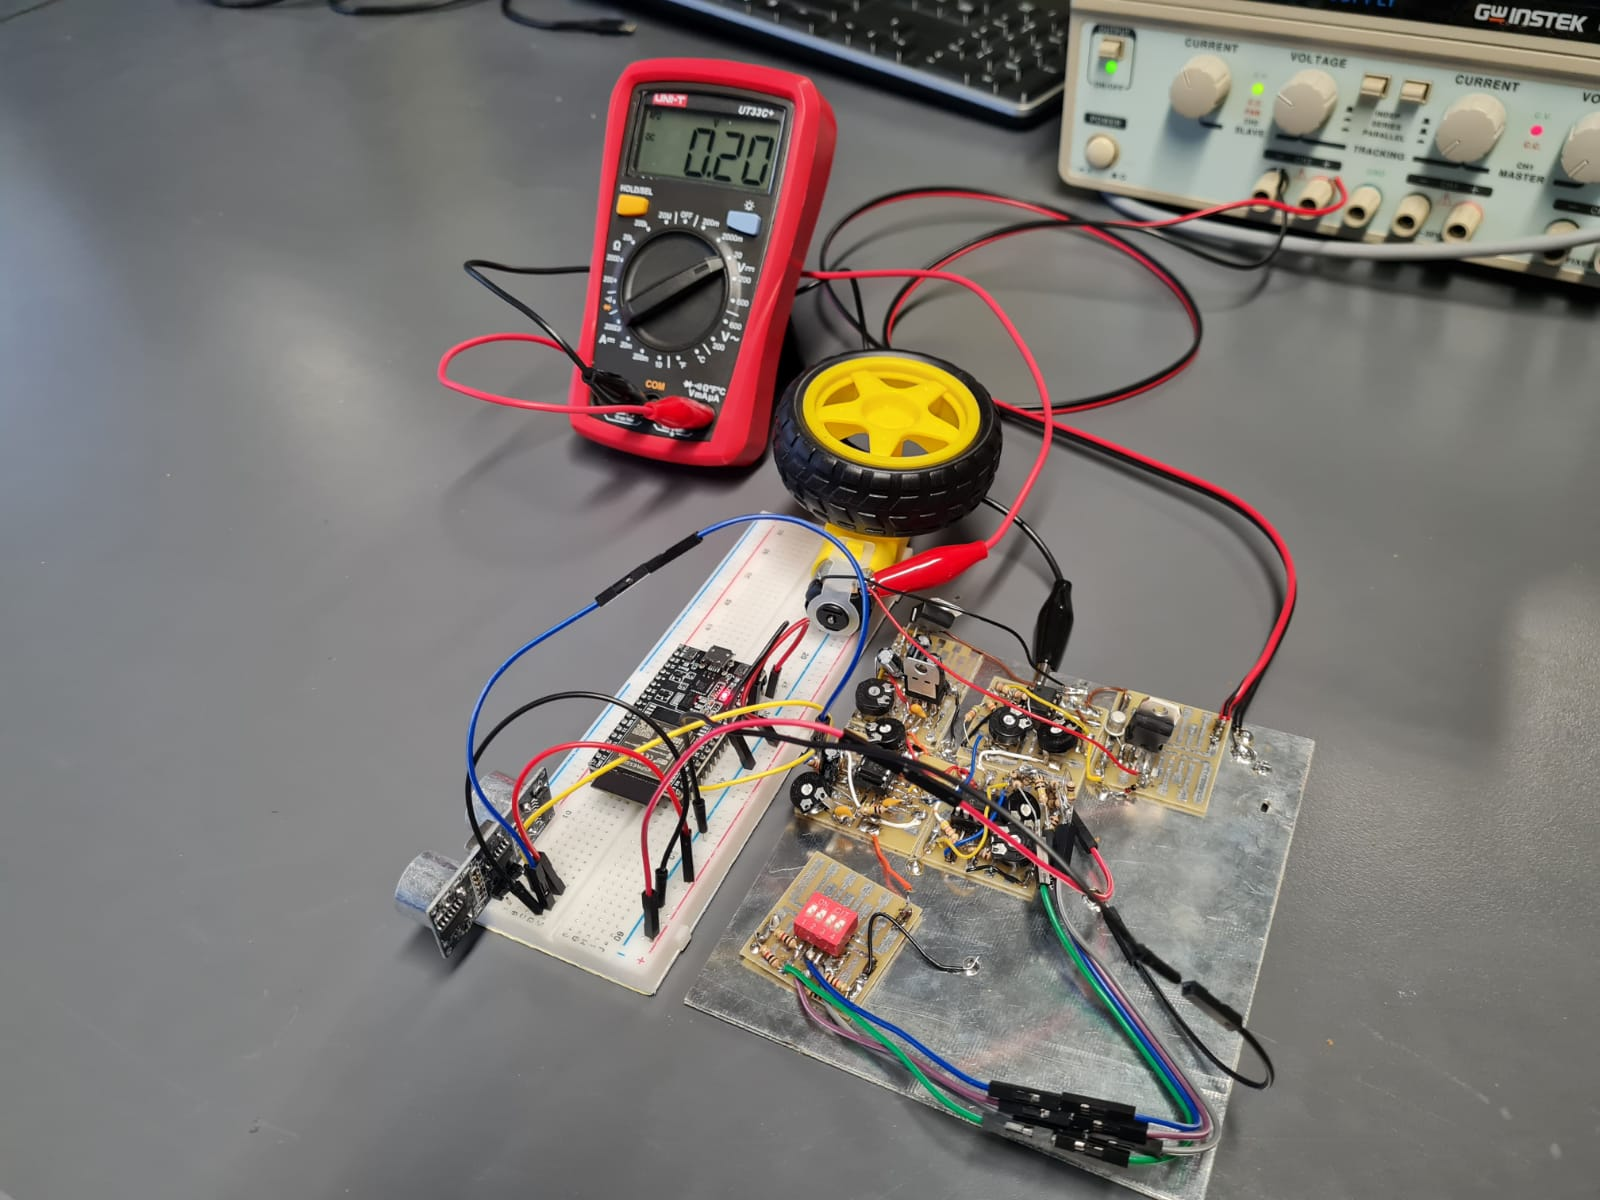
\includegraphics[width=1.0\linewidth]{motorController_far_0000}
        \captionof{figure}{Motor Voltage: Object Far, Speed 0000}
        \label{fig:motorController_far_0000}
    \end{minipage}
    \begin{minipage}{.38\textwidth}
        \centering
        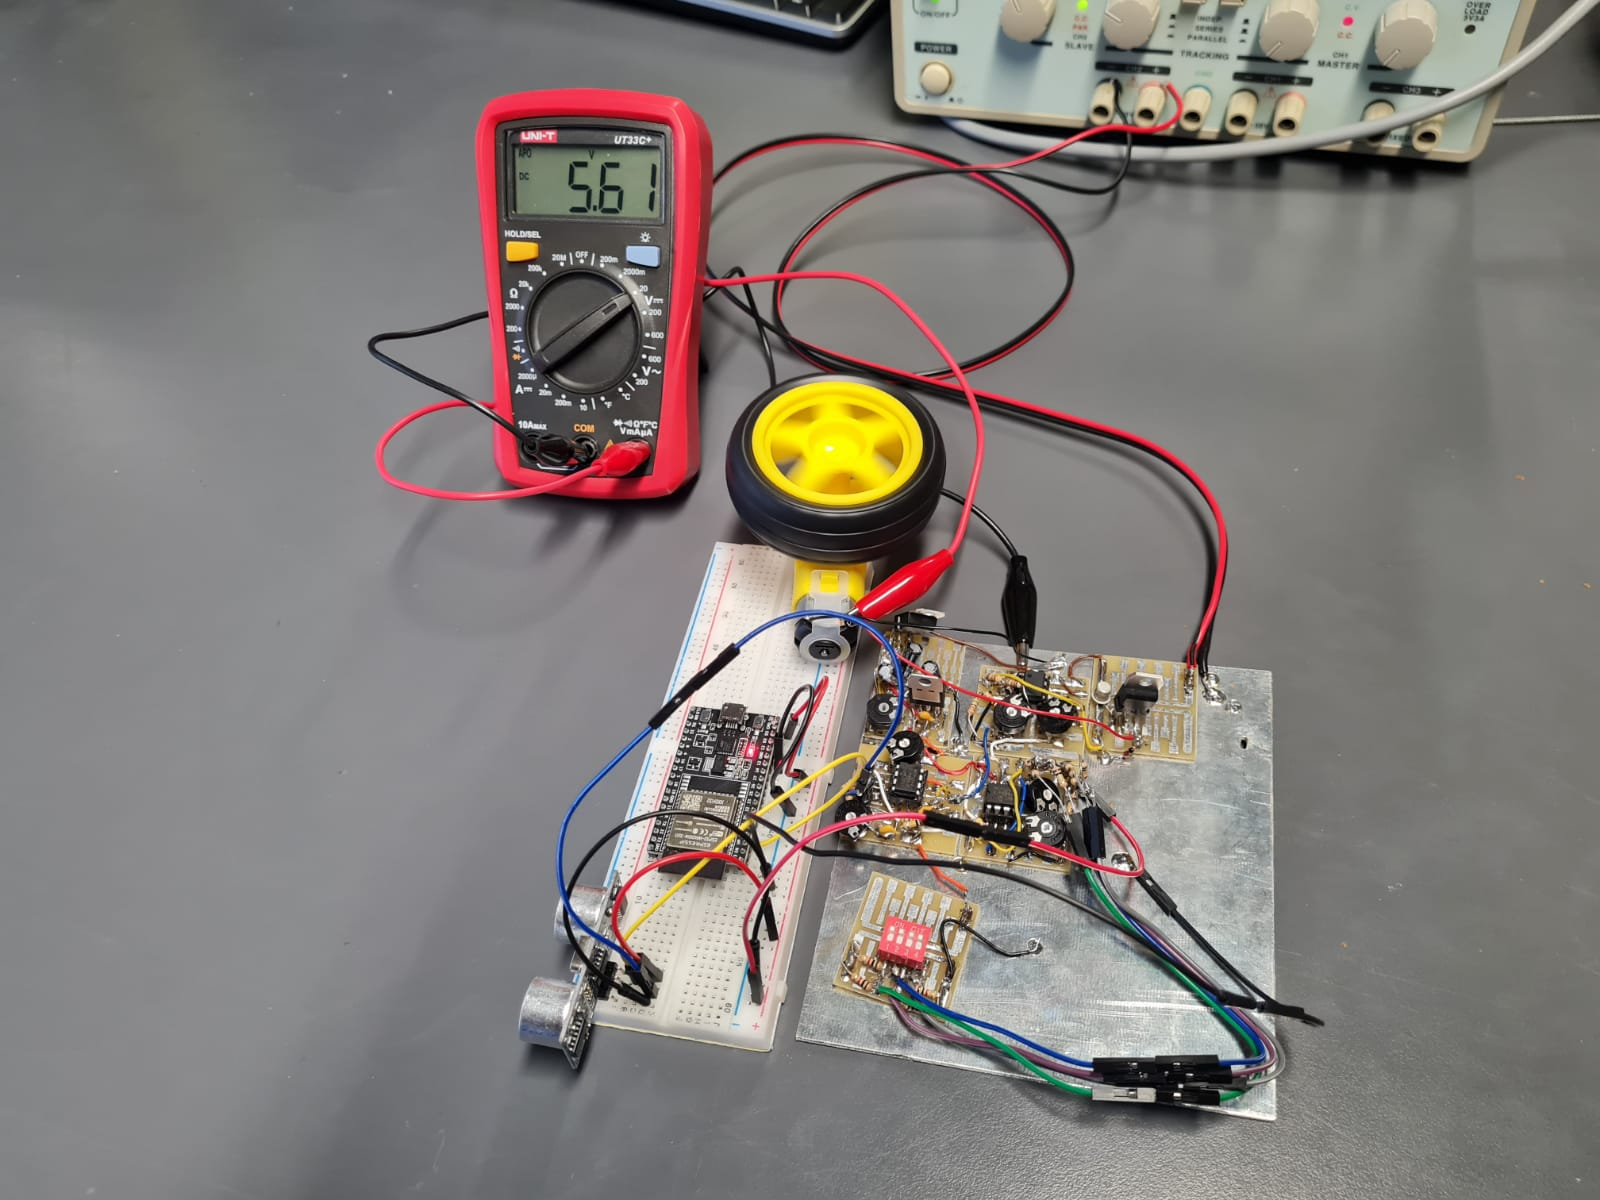
\includegraphics[width=1.0\linewidth]{motorController_far_1111}
        \captionof{figure}{Motor Voltage: Object Far, Speed 1111}
        \label{fig:motorController_far_1111}
    \end{minipage}
\end{figure}

\begin{figure}[!htb]
    \centering
    \begin{minipage}{.38\textwidth}
        \centering
        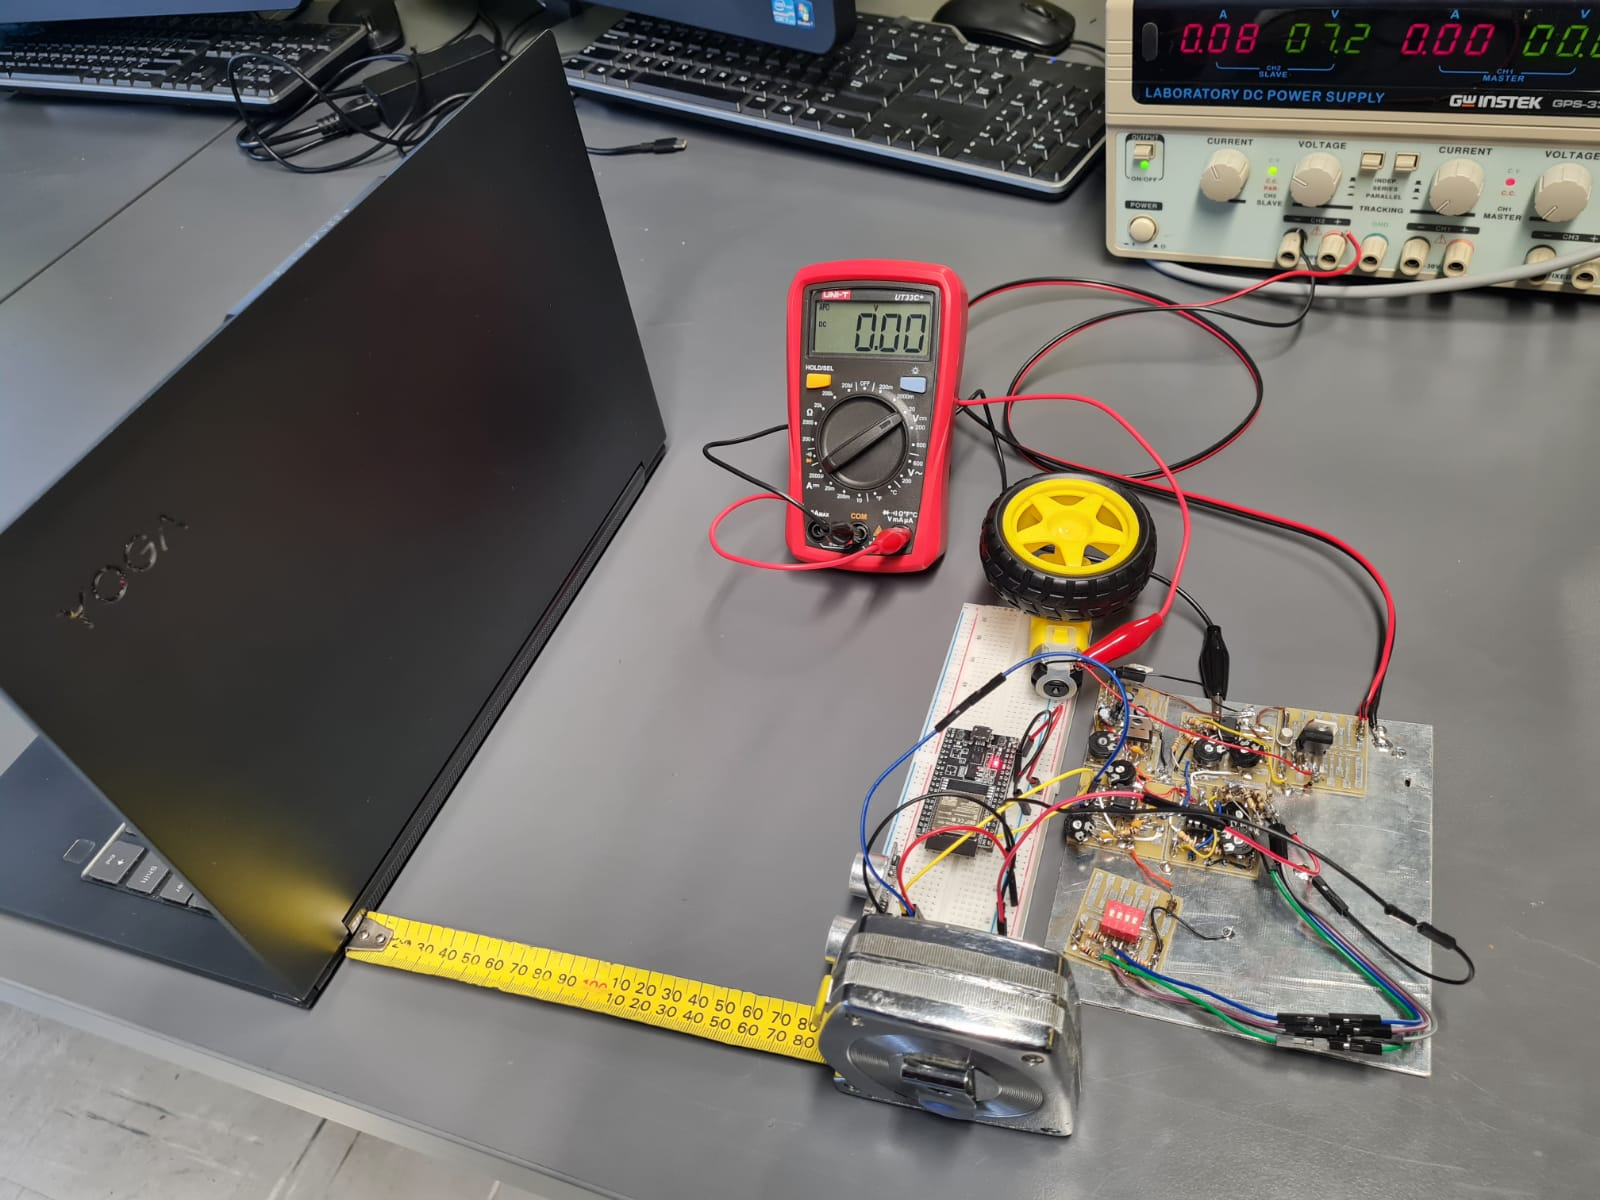
\includegraphics[width=1.0\linewidth]{motorController_near_0000}
        \captionof{figure}{Motor Voltage: Object Near, Speed 0000}
        \label{fig:motorController_near_0000}
    \end{minipage}
    \begin{minipage}{.38\textwidth}
        \centering
        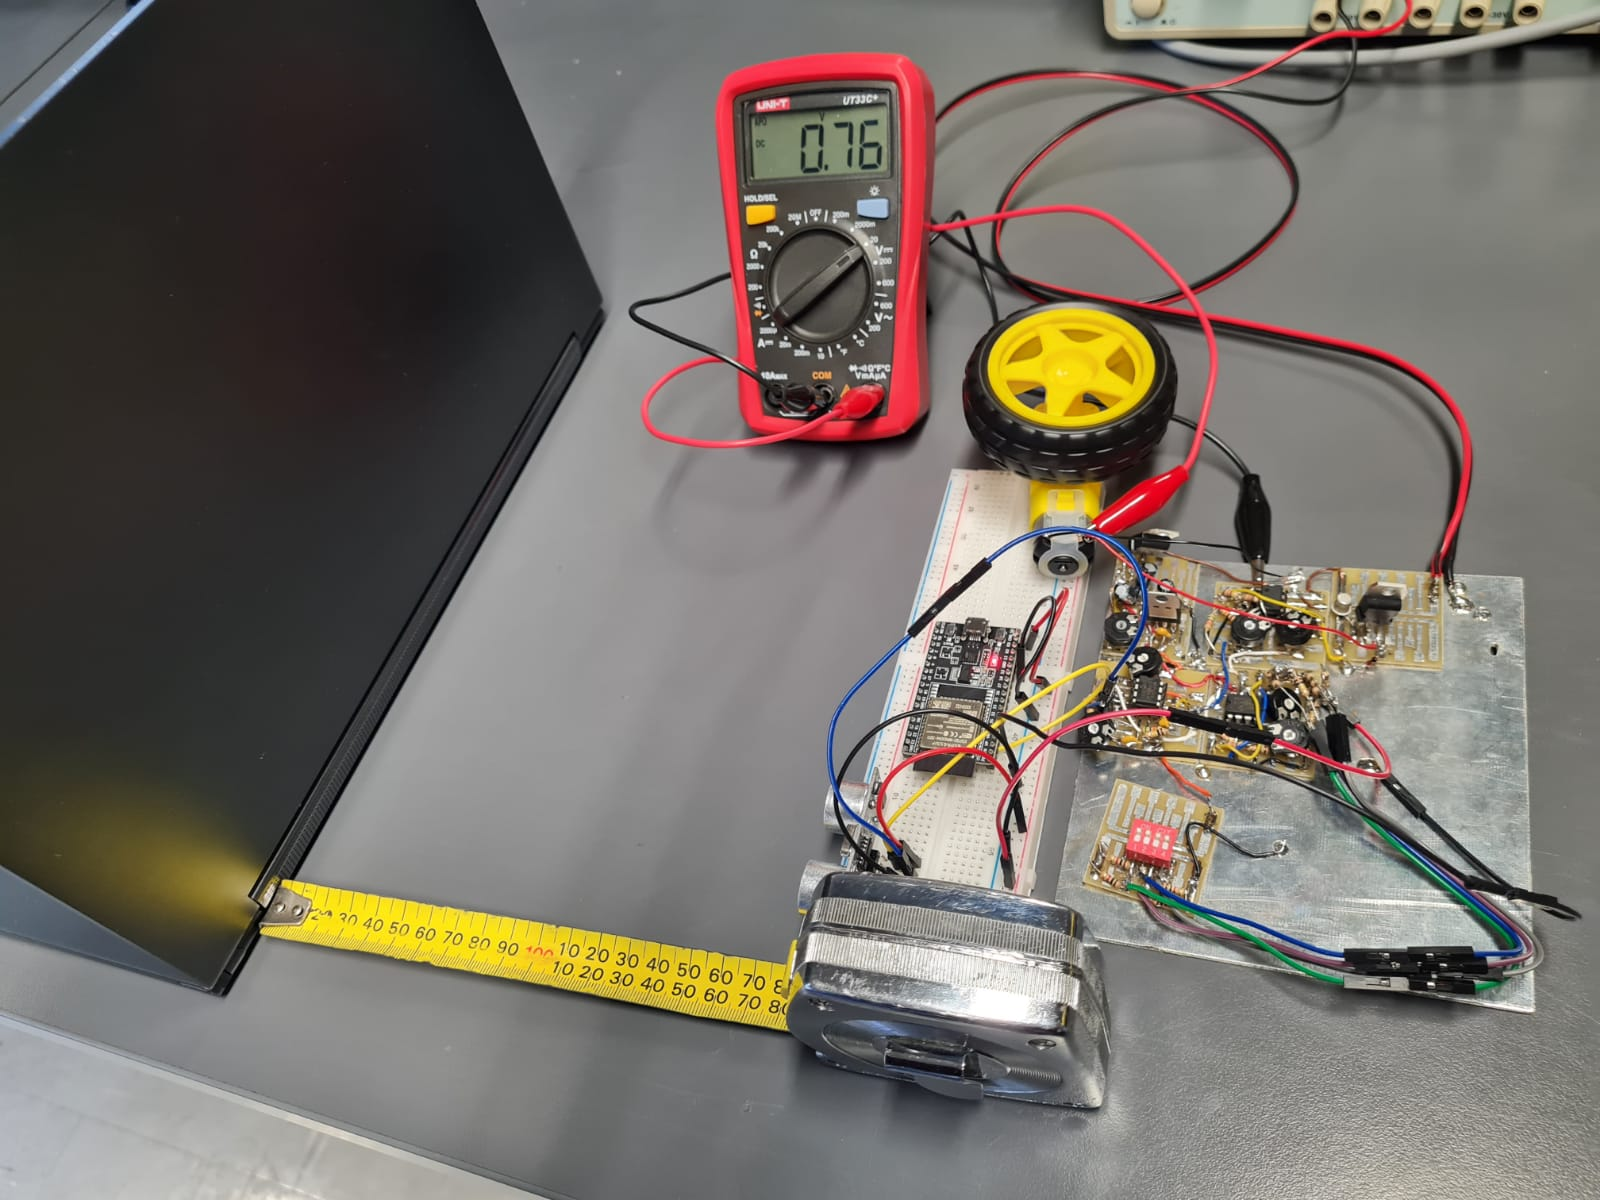
\includegraphics[width=1.0\linewidth]{motorController_near_1111}
        \captionof{figure}{Motor Voltage: Object Near, Speed 1111}
        \label{fig:motorController_near_1111}
    \end{minipage}
\end{figure}

The above four conditions show that the requirements were adhered to, in that the voltage is high $> \SI{5.5}{V}$
when the object is far and the torque command is a maximum, and the voltage is low $< \SI{0.5}{V}$ in all other edge-cases.

The designed $\SI{20}{cm}$ threshold was also measured, with the voltage resultant being $\SI{0.76}{V}$ as shown in Figure \ref{fig:motorController_20cm_1111}.
Although this was designed to equal 0.6 V at 20 cm, the motor is switched off at 0.76 V, and so the final requirement was still met.

\begin{figure}[!htb]
  \centering
  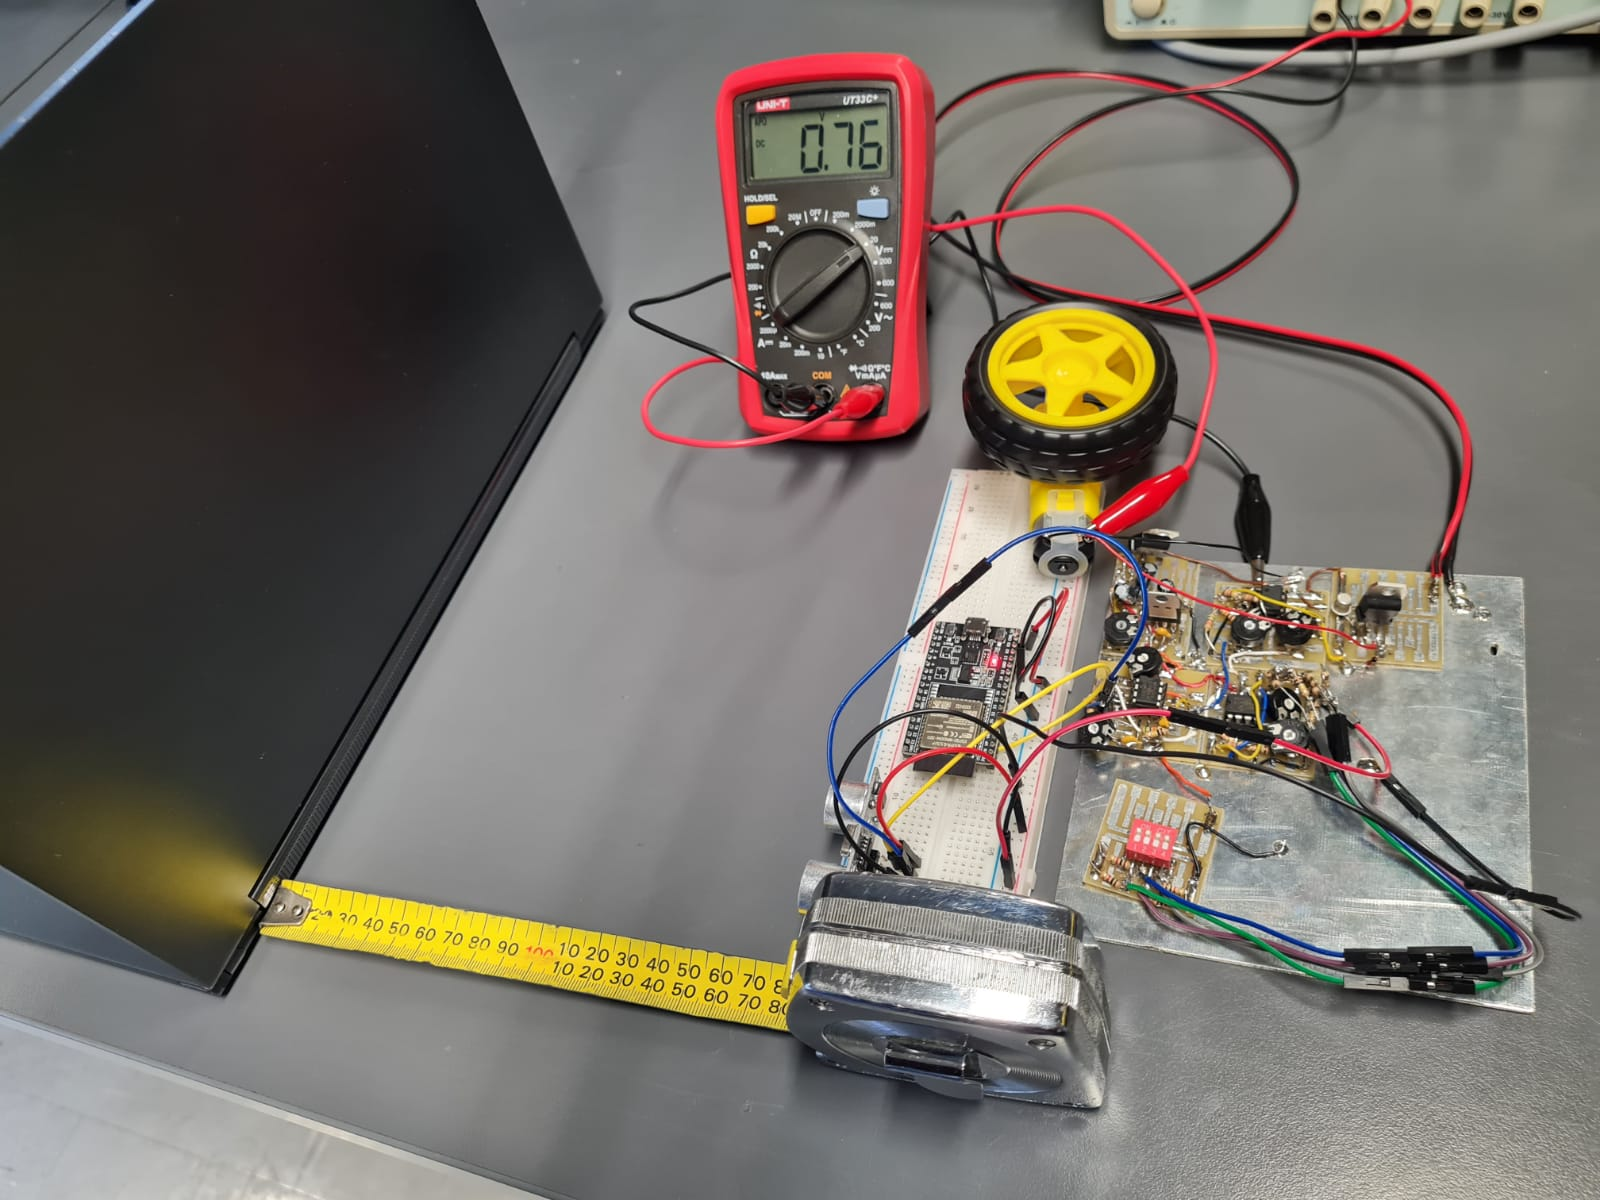
\includegraphics[width=0.3\textwidth]{motorController_20cm_1111}
  \caption{Motor Voltage: Object 20cm, Speed 1111}
  \label{fig:motorController_20cm_1111}
\end{figure}